\chapter{Materiał i metoda badawcza\@}
\label{ch:material-badawczy}

Przegląd literatury ukazuje obfitość raportów dotyczących identyfikacji choroby Parkinsona na podstawie krótkich fragmentów mowy, takich jak samogłoski, sylaby, czy krótkie słowa i zdania.
W tych badaniach wykorzystywane są różnorodne zadania wokalne, metody ekstrakcji cech oraz klasyfikacji.
Jednak wiele czynników wpływa na trudność obiektywnego porównania proponowanych rozwiązań, w tym różnice w wykorzystywanych bazach danych.

W niniejszej pracy przeprowadzono porównanie skuteczności wybranych architektur sieci konwolucyjnych oraz ocenić ich przydatność w diagnozowaniu choroby Parkinsona na podstawie różnych samogłosek.
Zastosowano  połączenie trzech różnych baz danych w celu poszerzenia zbioru o dodatkowe wzorce.

W tym rozdziale przedstawiono szczegółowy opis danych użytych do porównania efektywności i wydajności różnych algorytmów w diagnozowaniu choroby Parkinsona na podstawie mowy.
Omówiono proces przygotowania sygnałów oraz parametryzację sygnału akustycznego.
Następnie przedstawiono opis algorytmów, które zostały wykorzystane do realizacji postawionych zadań.
Schemat przyjętego podejścia został zilustrowany na Rys.~\ref{fig:methodology}.


\begin{figure}[htbp]
	\centering
	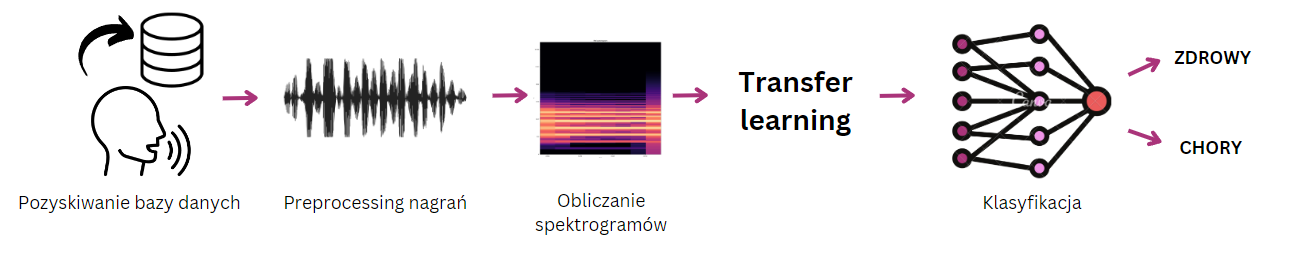
\includegraphics[width=1\textwidth]{./img/methodology}
	\caption{Schemat przyjętego podejścia\@}
    \label{fig:methodology}
\end{figure}

%---------------------------------------------------------------------------

\section{Materiał badawczy}
\label{sec:material-badawczy}

Materiałem badawczym w niniejszej pracy magisterskiej są nagrania głosowe podtrzymywanych samogłosek (ang. \emph{sustained vowels}) /a/, /e/, /i/, /o/ oraz /u/.
Baza danych obejmuje nagrania osób zdrowych oraz cierpiących na chorobę Parkinsona.
Podstawą skuteczności metod uczenia maszynowego jest odpowiednie przygotowanie danych, zarówno pod względem jakości, jak i ilości.
To kluczowy element, który wpływa na wydajność i zdolność modelu do radzenia sobie w rzeczywistym środowisku.
Dane użyte do trenowania modelu muszą być dokładne, spójne i reprezentatywne dla rzeczywistego środowiska, w którym będzie działał model.
Jest to podobne do procesu nauki lekarza – im więcej przypadków lekarz widzi i diagnozuje, tym lepiej radzi sobie z różnymi przypadkami w praktyce.
W  uczeniu maszynowym większa ilość danych pozwala na uchwycenie różnic międzyosobniczych i niuansów w danych, co przekłada się na większą stabilność i skuteczność modelu.
Model musi być w stanie radzić sobie z nowymi danymi, które nie były używane podczas treningu.

W pracy wykorzystano dane, zarejestrowane dla 3 różnych języków: polskiego, włoskiego oraz hiszpańskiego.
Wykorzystanie baz danych uwzględniając różne grupy językowe pozwala na analizę uniwersalności narzędzia służącego do automatycznej diagnozy choroby Parkinsona, tak by nie było ono ograniczone tylko do jednej grupy narodowościowej czy geograficznej.
Takie podejście pozwala na utworzenie modelu uniwersalnego, który mógłby być używany na skalę międzynarodową przyczyniając się do poprawy jakości opieki zdrowotnej i diagnozy tej choroby.

Warto też zauważyć, że żadna z dostępnych publicznie baz danych nie zawiera wystarczającej ilości nagrań, by mówić o stabilnym rozwiązaniu, które mogłoby zostać użyte na szeroką skalę.
Łączenie zestawów danych może znacząco poprawić zdolności generalizacyjne modelu.

\subsection{Baza danych w języku polskim}
\label{subsec:polska-baza}

Materiał badawczy pochodzący od osób cierpiących na chorobę Parkinsona (PD) i posługujących się językiem polskim, został zgromadzony w ramach
realizacji rozprawy doktorskiej we współpracy z Krakowskim Szpitalem Specjalistycznym im.
Jana Pawła II~\cite{daria:2018}.
W bazie danych znajdują się nagrania samogłosek /a/, /e/, /i/, /o/ oraz /u/ z wydłużoną intonacją, pozyskane od 27 pacjentów.
Dla każdego z pacjentów dostępne jest jedno nagranie każdej z wymienionych samogłosek.
W ramach przeprowadzonych badań pomiary zostały wykonane przed spożyciem leków oraz w określonych odstępach czasowych po podaniu lewodopy.
Przed każdym pomiarem lekarz neurolog przeprowadzał badanie pacjenta i oceniał jego stan, wykorzystując skalę UPDRS\@.
W niniejszej pracy magisterskiej wykorzystano jedynie nagrania głosowe zarejestrowane przed podaniem leku.

Nagrania osób zdrowych zostały zebrane w ramach tej pracy magisterskiej przy wykorzystaniu aplikacji \emph{Easy Voice Recorder}.
Ustalono protokół nagrywania, wykluczając osoby poniżej 50 roku życia, palące oraz ze zdiagnozowaną lub podejrzewaną chorobą wpływającą na aparat mowy, lub korę mózgową (np.
choroba Parkinsona, epilepsja, padaczka).
Pozyskiwano nagrania jedynie od osób, dla których językiem ojczystym jest polski.
Każda osoba kwalifikująca się do badania otrzymała zadanie trzykrotnego wypowiedzenia samogłosek /a/, /e/, /i/, /o/ oraz /u/ w odstępach czasowych, utrzymując dźwięk przez co najmniej 2 sekundy.
Następnie nagrania zostały dokładnie przeanalizowane.
Usunięto nagrania zbyt krótkie oraz te, które nie spełniały kryteriów dotyczących jakości.
Otrzymana baza danych nadal zawierała nagrania od 27 osób chorych oraz od 26 osób zdrowych, zmieniła się jedynie liczebność nagrań dla poszczególnych samogłosek.
W tabeli~\ref{tab:polish_database} przedstawiono informacje dotyczące bazy danych.

\begin{table}[h]
\centering
\caption{Charakterystyka polskiej bazy danych}
\label{tab:polish_database}
\begin{tabular}{|l|c|c|c|}
\hline
\textbf{Kategoria} &\textbf{Osoby zdrowe (HC)} &\textbf{Osoby chore (PD)} &\textbf{Razem} \\ \hline
Liczba osób &26 &27 &53\\ \hline
Liczba nagrań &67 &27 &94\\ \hline
Średnia wieku &60,88 ± 7,98 &64,49 ± 8,49  &62,68 ± 8,43\\ \hline
Liczba kobiet &18 &13 &31\\ \hline
Liczba mężczyzn &8 &14 &22 \\ \hline
\end{tabular}
\end{table}

\subsection{Baza danych w języku włoskim}
\label{subsec:wloska-baza}

Włoska baza danych to \emph{Italian Parkinson's Voice And Speech}, która dostępna jest na platformie \emph{IEEEDataPort}~\cite{italian-database}.
Zbiór zawiera wiele różnych podzbiorów, ale wykorzystano jedynie podtrzymywane samogłoski /a/, /e/, /i/, /o/ oraz /u/.
Ocena stopnia zaawansowania choroby została przeprowadzona przy pomocy skali UPDRS\@.
Wszystkie nagrania pochodzą od osób, dla których natywnym językiem jest włoski.
Początkowo baza danych zawiera nagrania od 50 osób, jednak po wstępnym oczyszczeniu wykorzystano jedynie 45.
Charakterystykę zbioru przedstawiono w tabeli~\ref{tab:italian-database}

\begin{table}[h]
\centering
\caption{Charakterystyka włoskiej bazy danych}
\label{tab:italian-database}
\begin{tabular}{|l|c|c|c|}
\hline
\textbf{Kategoria} &\textbf{Osoby zdrowe (HC)} &\textbf{Osoby chore (PD)} &\textbf{Razem} \\ \hline
Liczba osób &19 &26 &45\\ \hline
Liczba nagrań &38 &52 &90\\ \hline
Średnia wieku &67,31 ± 5,23 &66,96 ± 8,59  & 67,11 ± 7,36 \\ \hline
Liczba kobiet &10 &7 &17\\ \hline
Liczba mężczyzn &9 &19 &28 \\ \hline
\end{tabular}
\end{table}


\subsection{Baza danych w języku hiszpańskim}
\label{subsec:hiszpanska-baza}


Hiszpańska baza danych (PC-GITA) ~\cite{pc-gita} zawiera nagrania mowy 50 pacjentów z PD i tyle samo osób zdrowych, dopasowanych pod względem wieku i płci.
Wszyscy uczestnicy posługują się kolumbijską odmianą języka hiszpańskiego, a nagrania zostały zebrane zgodnie z protokołem uwzględniającym wymagania techniczne oraz zalecenia ekspertów z dziedzin lingwistyki, foniatrii i neurologii.
Kolekcja obejmuje takie zadania jak podtrzymywane wymawianie samogłosek, ocenę diadokokinetyczną, 45 słów, 10 zdań, tekst do czytania i monolog.
Podobnie jak w przypadku pozostałych baz wykorzystano jedynie nagrania samogłosek /a/, /e/, /i/, /o/ oraz /u/.
Na jednego uczestnika przypadają trzy powtórzenia każdej z samogłosek.
Szczegółowa charakterystyka zbioru została przedstawiona w tabeli~\ref{tab:spanish-database}

\begin{table}[ht]
\centering
\caption{Charakterystyka hiszpańskiej bazy danych}
\label{tab:spanish-database}
\begin{tabular}{|l|c|c|c|}
\hline
\textbf{Kategoria} &\textbf{Osoby zdrowe (HC)} &\textbf{Osoby chore (PD)} &\textbf{Razem} \\ \hline
Liczba osób &50 &50 &100\\ \hline
Liczba nagrań &150 &150 &300\\ \hline
Średnia wieku &60,90 ± 9,37 &61,14 ± 9,51  &61,02 ± 9,15\\ \hline
Liczba kobiet &25 &25 &50\\ \hline
Liczba mężczyzn &25 &25 &50 \\ \hline
\end{tabular}
\end{table}

\section*{}
Połączenie baz danych było możliwe ze względu na uniwersalność podstawy diagnostycznej, jaką są podtrzymywane samogłoski.
Nagrania różniły się długością, jednak wykorzystano jedynie krótkie fragmenty (0,1 s), więc nie stanowiło to problemu.
Wszystkie zostały zarejestrowane z częstotliwością próbkowania 44,1 kHz.

Trudno nie zauważyć znaczącej przewagi liczby nagrań w bazie hiszpańskojęzycznej (Rys.~\ref{fig:language-distribution}).
Jednak zrezygnowano z wyrównywania liczby nagrań w poszczególnych językach, z uwagi na to, że baza danych jest już stosunkowo niewielka, i dodatkowe ograniczenie liczby nagrań mogłoby znacząco zmniejszyć jej wartość i możliwości badawcze.
Zachowano zbliżone proporcje wieku (różnica w średniej wieku mniejsza niż 5 lat) i płci pomiędzy grupą pacjentów a grupą porównawczą.
Drobne różnice w liczbie próbek w poszczególnych przedziałach wiekowych nie powinny mieć istotnego wpływu na wyniki klasyfikacji.
Liczba nagrań dla każdej samogłoski została wyrównana, tak by umożliwić obiektywne porównanie ich potencjalnego wykorzystania.
Szczegółowe charakterystyki zbioru danych zostały przedstawione na Rys.~\ref{fig:charakterystyka-bazy}.


\begin{figure}
    \begin{subfigure}{0.9\textwidth}
        \centering
       	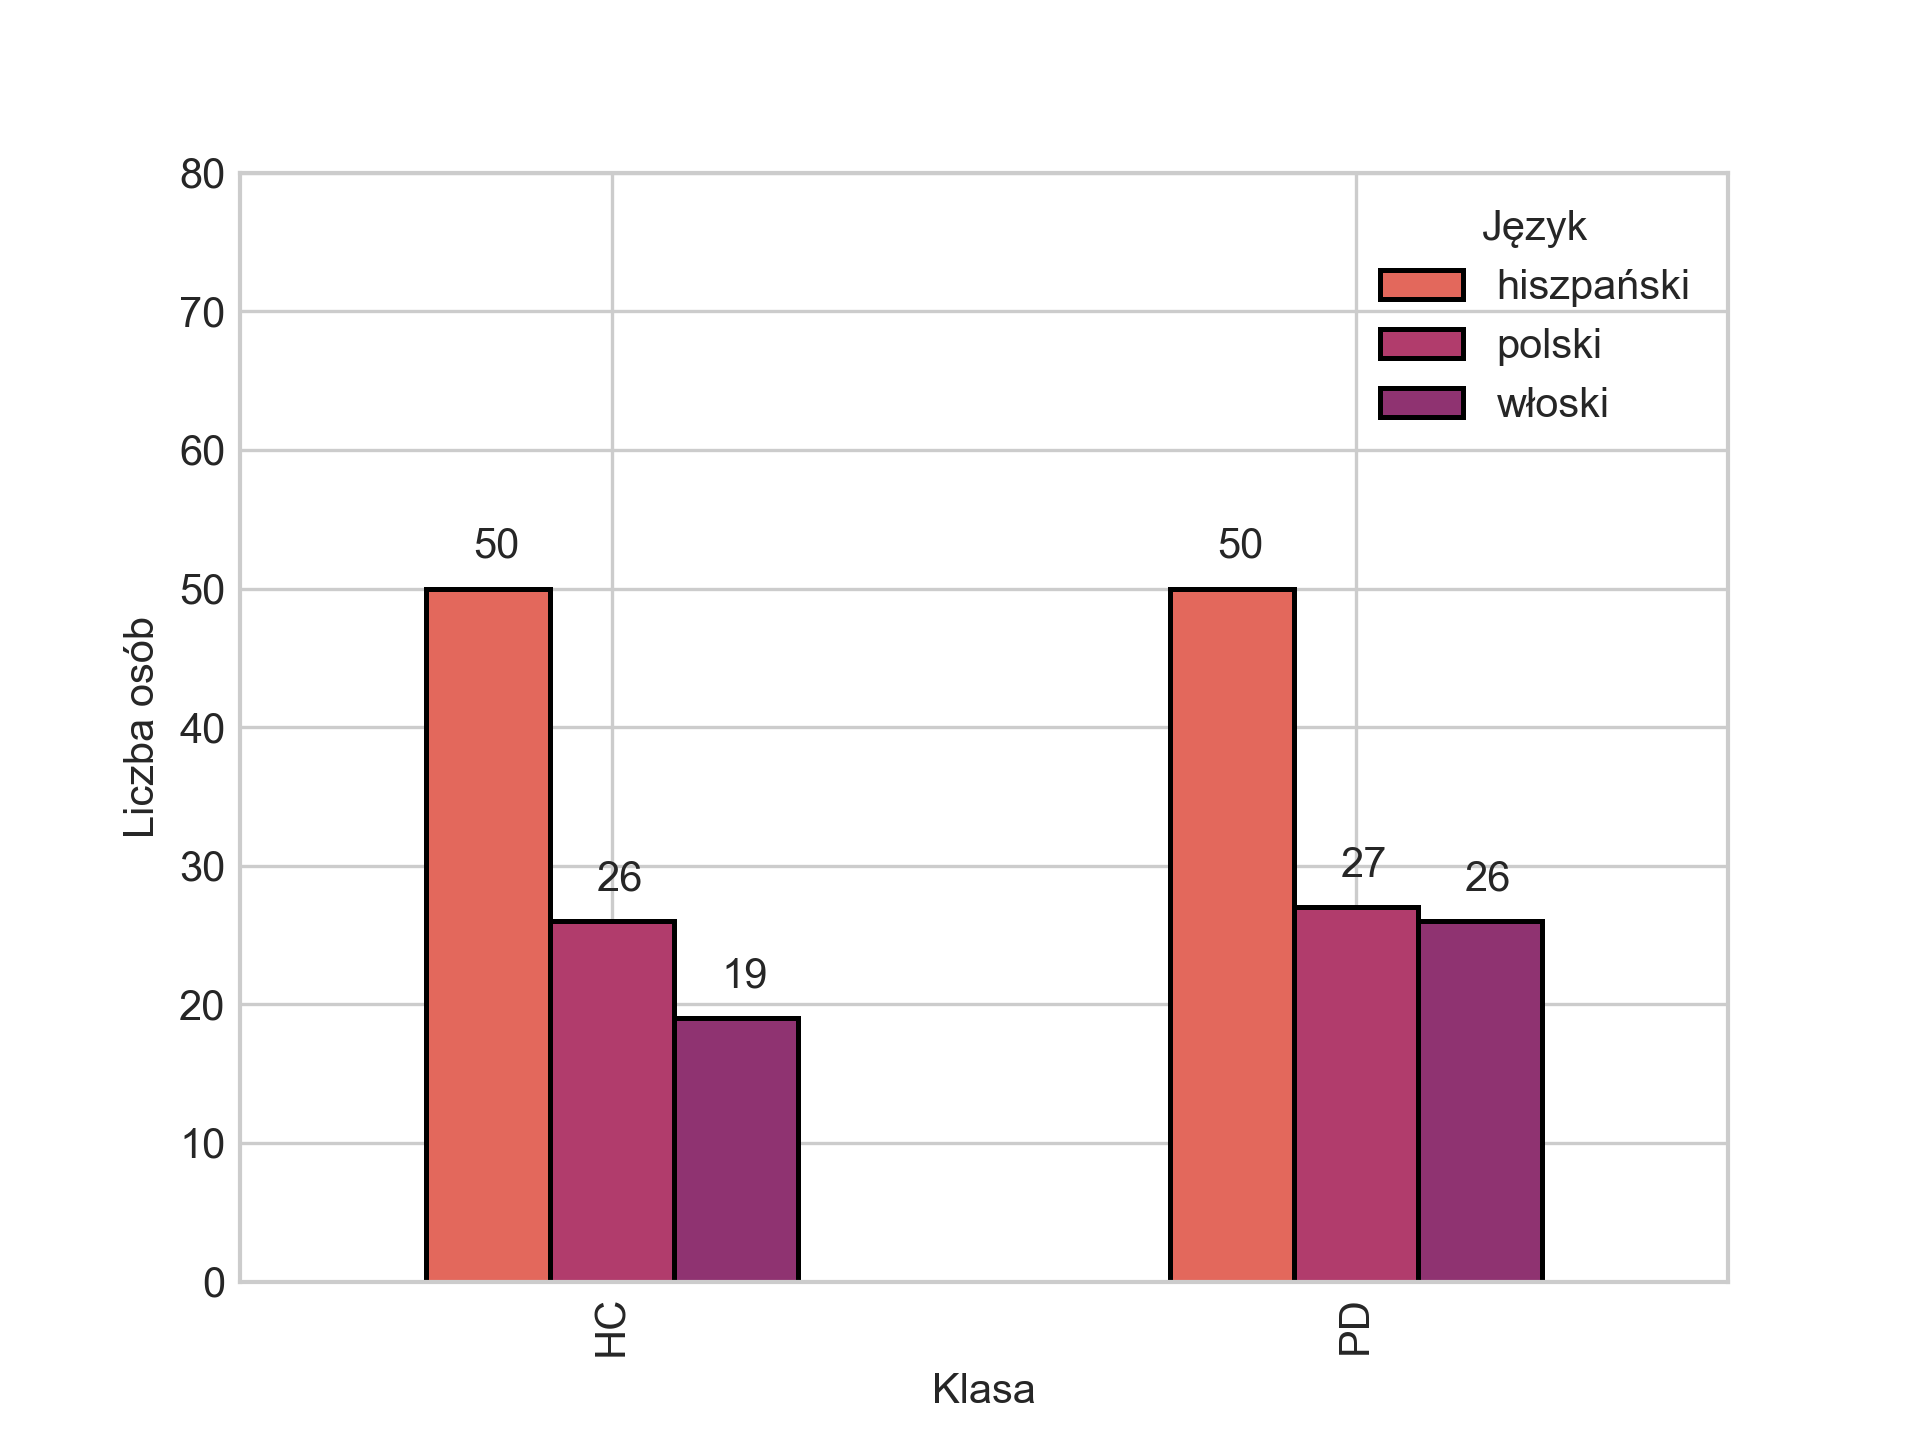
\includegraphics[width=0.60\textwidth]{./img/database stats/languages_distribution}
	    \caption{Udział nagrań z poszczególnych grup językowych}
        \label{fig:language-distribution}
    \end{subfigure}

    \begin{subfigure}{0.85\textwidth}
        \centering
        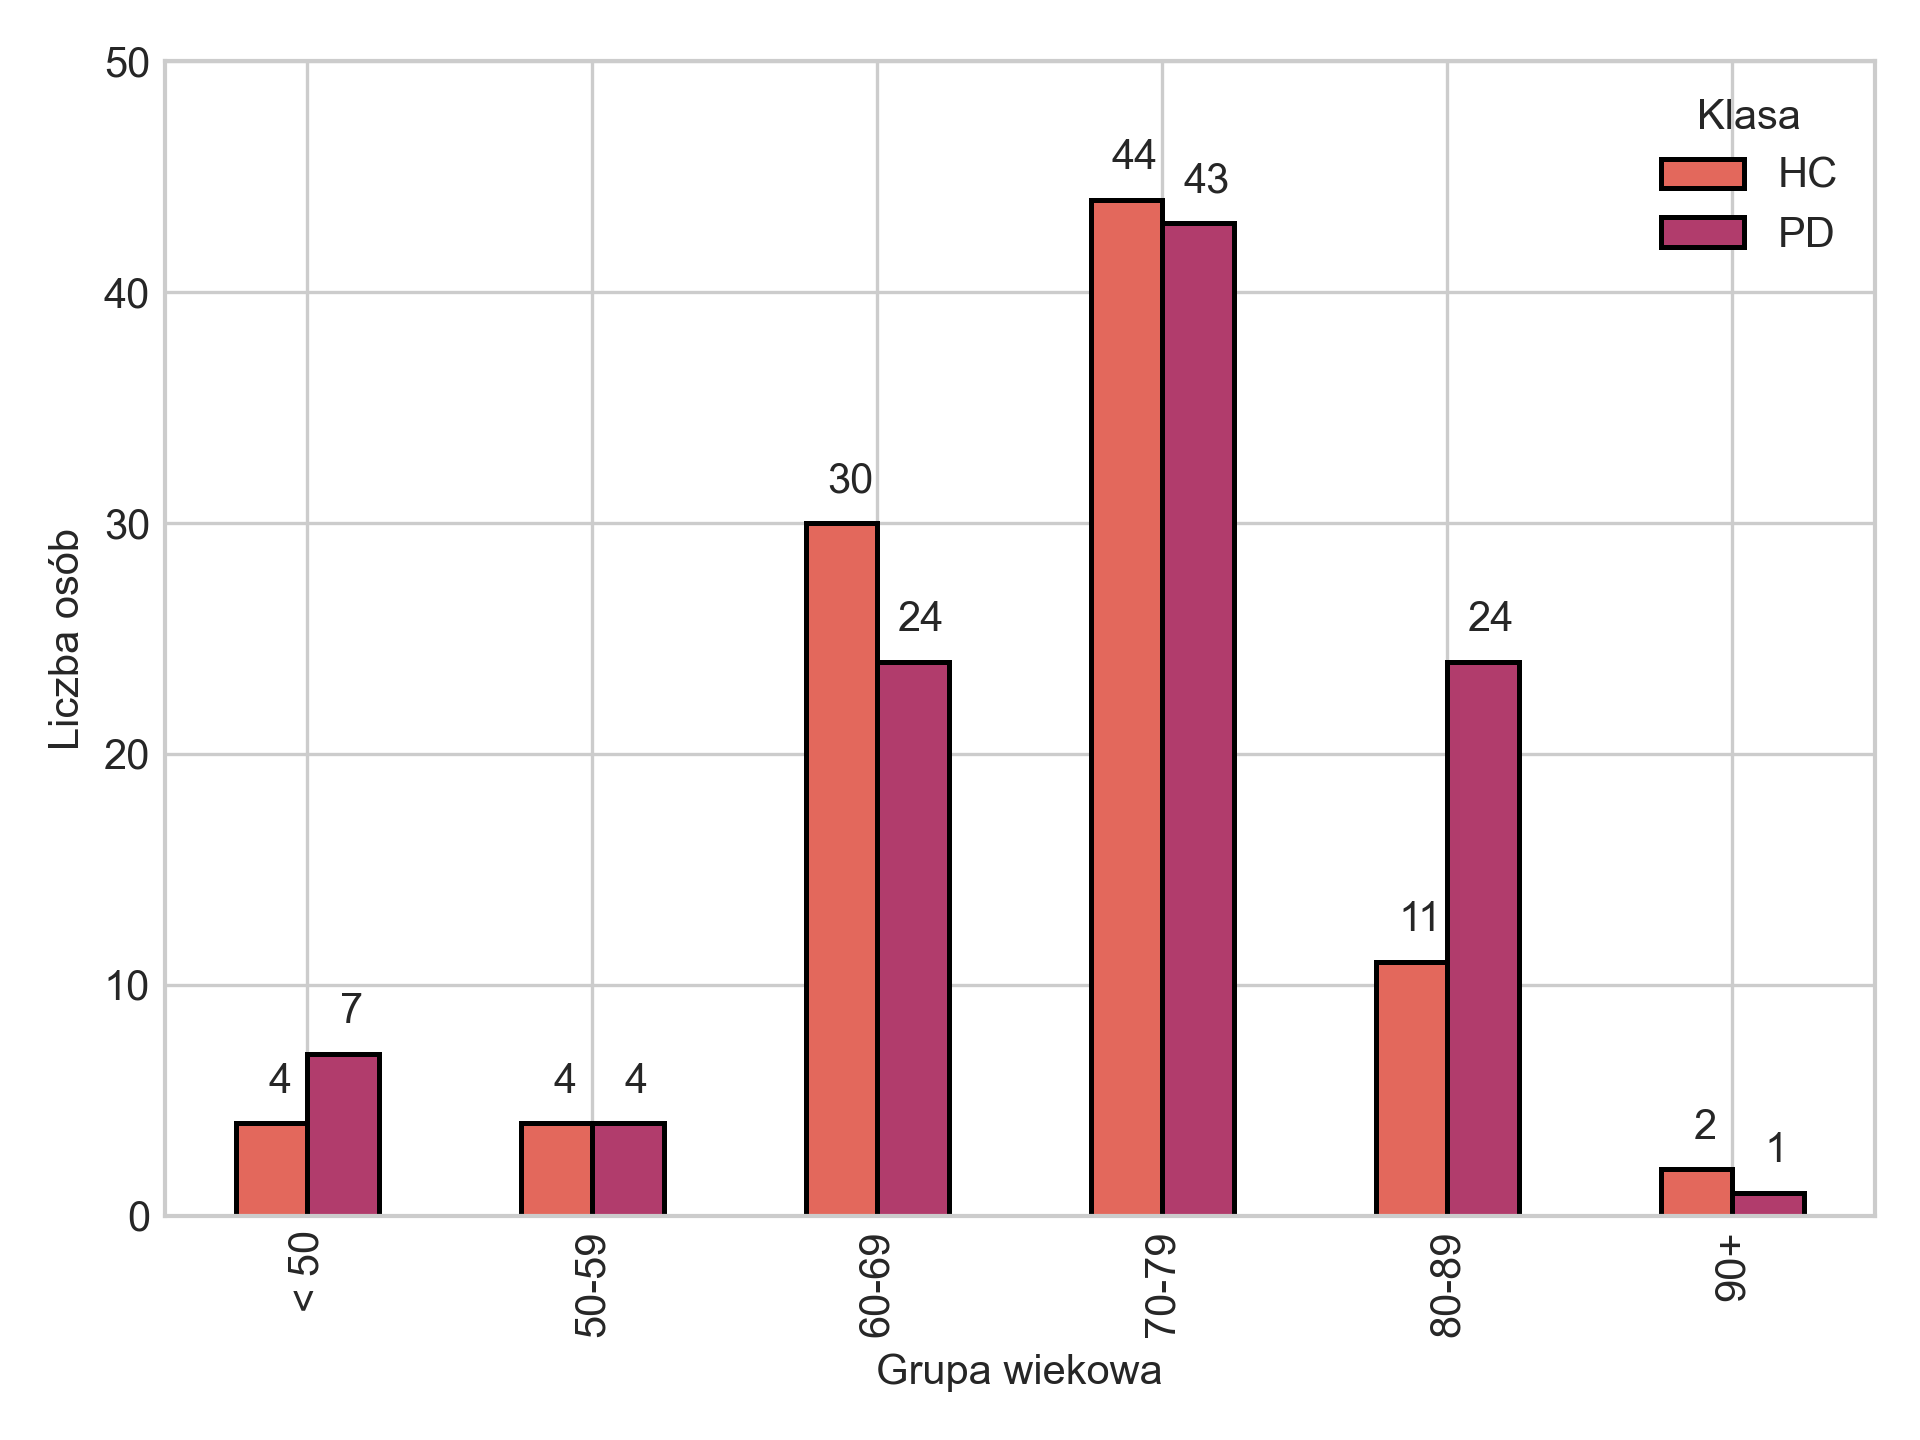
\includegraphics[width=0.60\textwidth]{./img/database stats/age_distribution}
        \caption{Rozkład grup wiekowych w poszczególnych klasach}
        \label{fig:age-distribution}
    \end{subfigure}

    \begin{subfigure}{0.85\textwidth}
        \centering
       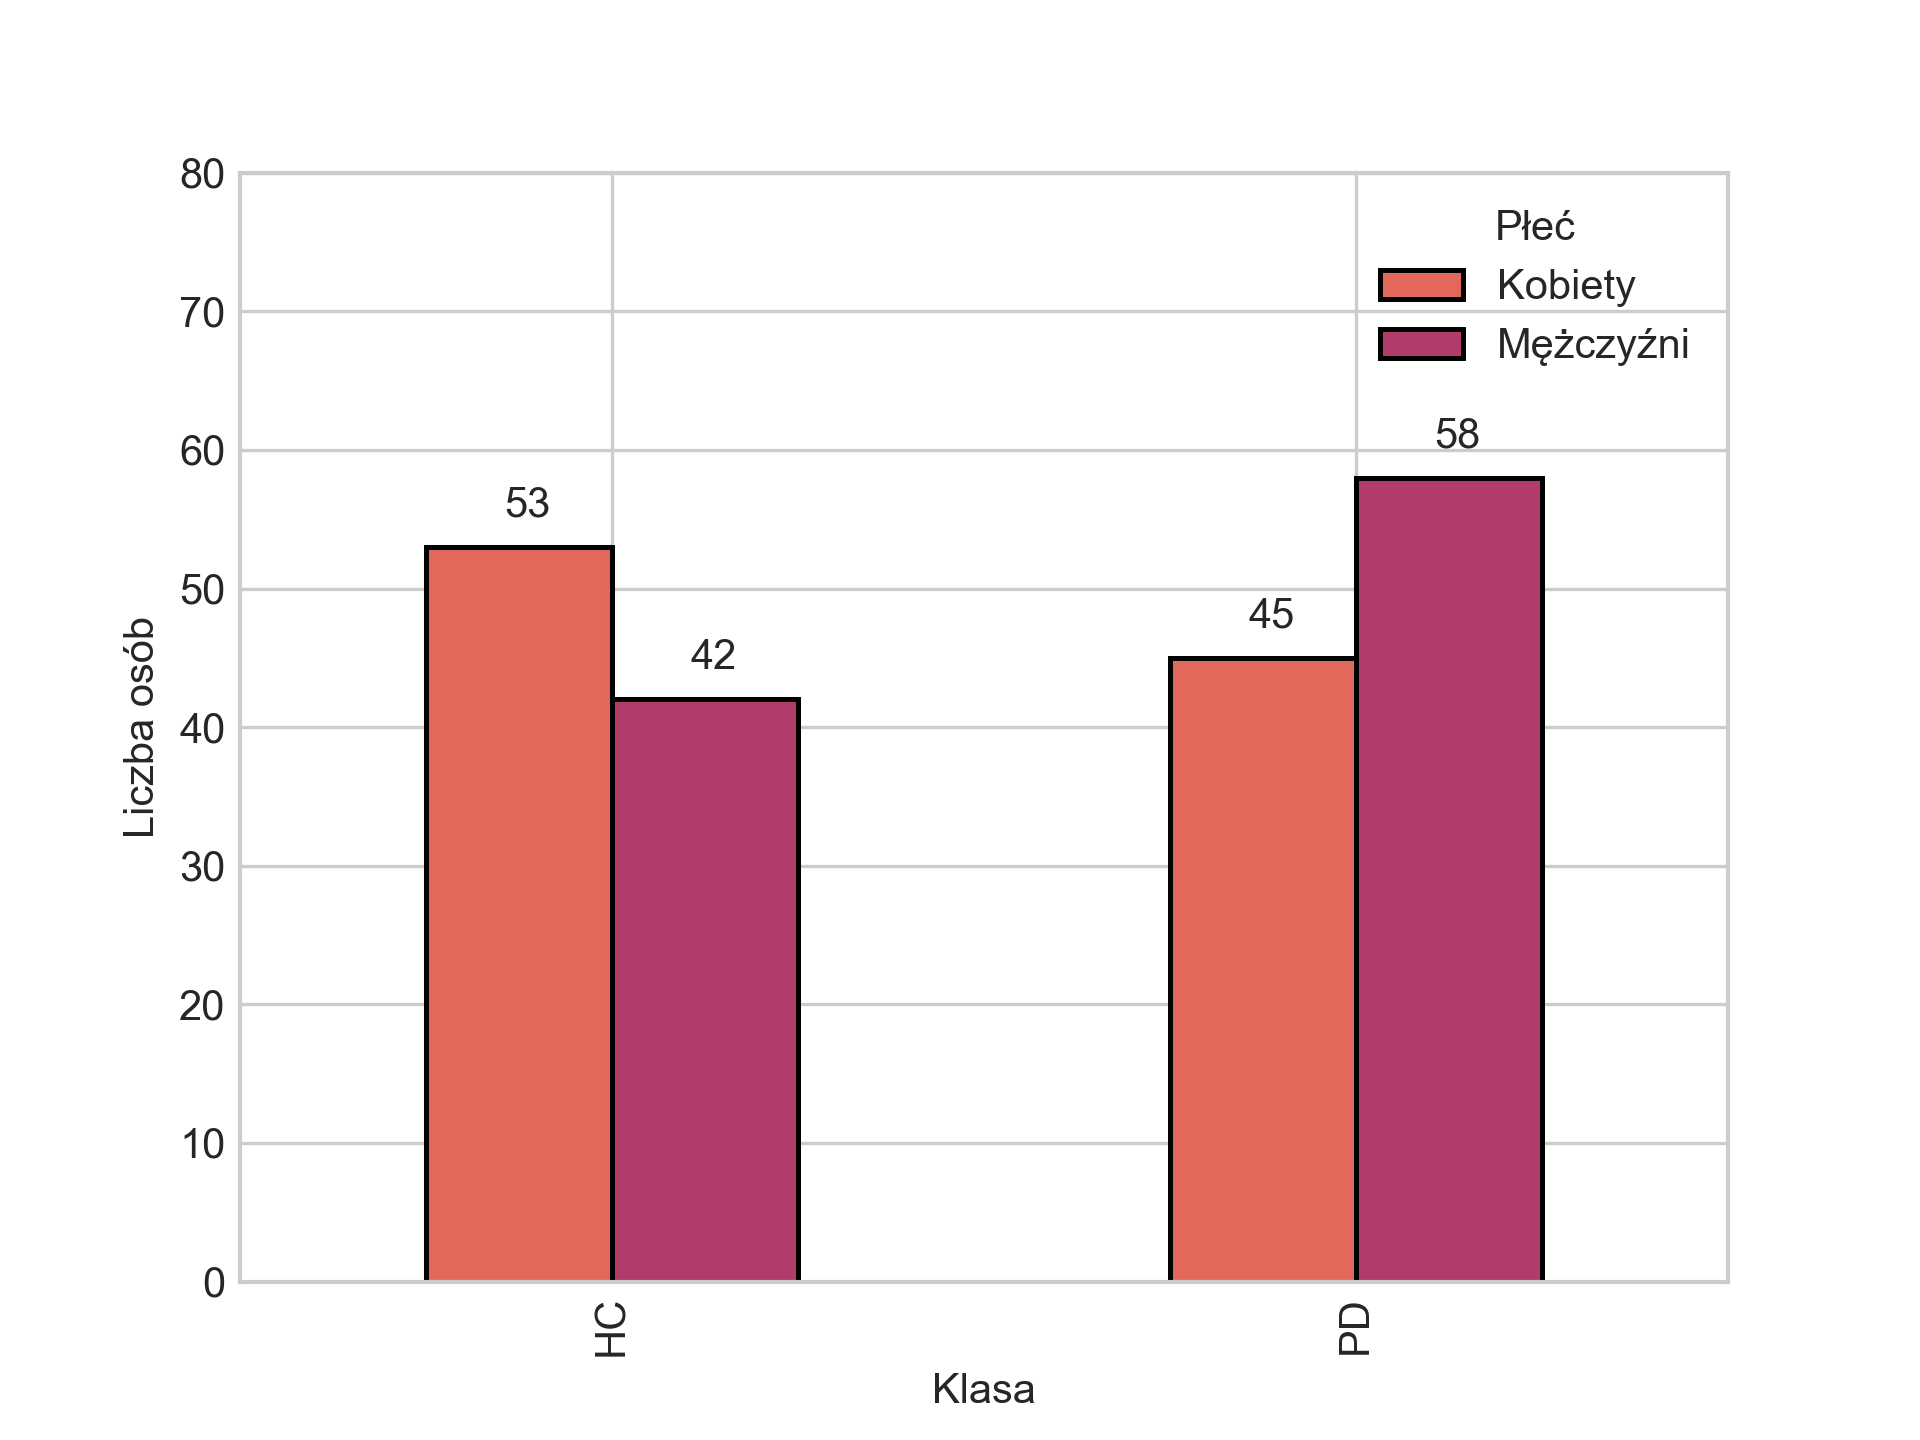
\includegraphics[width=0.65\textwidth]{./img/database stats/gender_distribution}
	    \caption{Rozkład płci w klasach}
        \label{fig:gender-distribution}
    \end{subfigure}

    \caption{Charakterystyka wykorzystanej bazy danych. (a) stosunek liczby osób z poszczególnych grup językowych;
        (b) rozkład wiekowy w grupie osób z chorobą Parkinsona i grupie osób zdrowych; (c) rozkład płci w grupie osób z PD i grupie osób zdrowych.}
    \label{fig:charakterystyka-bazy}
\end{figure}



\begin{table}[h]
\centering
\caption{Charakterystyka stworzonej bazy danych}
\label{tab:summary-database}
\begin{tabular}{|l|c|c|c|}
\hline
\textbf{Kategoria} &\textbf{Osoby zdrowe (HC)} &\textbf{Osoby chore (PD)} &\textbf{Razem} \\ \hline
Liczba osób &95 &103 &198\\ \hline
Liczba nagrań &255 &229 &484\\ \hline
Średnia wieku & 62,18 ± 8,70 & 62,84 ± 9,45  & 62,32 ± 8,99 \\ \hline
Liczba kobiet &53 &45 &98\\ \hline
Liczba mężczyzn &42 &58 &100 \\ \hline
\end{tabular}
\end{table}
%---------------------------------------------------------------------------

\section{Parametryzacja sygnału akustycznego}
\label{sec:parametryzacja-sygnalu-akustycznego}

W kontekście projektowania rozwiązań związanych z uczeniem maszynowym, jednym z kluczowych aspektów jest staranne przygotowanie danych.
Proces ten jest niezwykle istotny i obejmuje kilka kluczowych etapów, które mają ogromny wpływ na jakość i skuteczność modelu.
Dwa główne etapy, które wymagają szczególnej uwagi, to preprocessing i ekstrakcja cech.
Preprocessing odnosi się do przetwarzania wstępnego danych dźwiękowych przed ich podaniem modelowi uczenia maszynowego.
W ramach tego procesu usuwane są zakłócenia, szumy i niepożądane.
W przypadku nagrań może to obejmować filtrację, normalizację głośności, usuwanie niepotrzebnych fragmentów dźwięku oraz inne techniki poprawiające jakość sygnału.
Poprawne wykonanie etapu preprocessingu może znacząco wpłynąć na  jakość wyników uzyskiwanych przez modele.
Drugim istotnym etapem jest ekstrakcja cech.
W ramach tego procesu z nagrań mowy wydobywane są istotne parametry lub cechy, które mogą być używane przez modele uczenia maszynowego do rozpoznawania wzorców.
Wybór odpowiednich cech i ich dokładna ekstrakcja mają kluczowe znaczenie, ponieważ to od nich zależy, jakie informacje zostaną dostarczone modelowi do analizy.

\subsection{Przygotowanie nagrań}
\label{subsec:preprocessing}

Nagrania zostały przycięte, tak by nie zawierały początkowych i końcowych fragmentów ciszy.
Ten proces eliminuje niepotrzebne fragmenty i skupia analizę jedynie na istotnych fragmentach mowy, co może poprawić skuteczność modelu.
W celu automatycznego usunięcia niepożądanych fragmentów skorzystano z pakietu \emph{Librosa} do, a następnie każde z nagrań zostało przeanalizowane w programie \emph{Audacity}.
Upewniono się, że nagrania zostały poprawnie przetworzone oraz wprowadzono ręcznie ewentualne poprawki.

Z uwagi na wykorzystanie różnych baz danych, charakteryzujących się zróżnicowanymi warunkami nagrywania, zdecydowano się na ograniczenie wpływu otoczenia na dokładność klasyfikacji.
W tym celu zastosowano filtr pasmowoprzepustowy, który pozwolił na eliminację niepotrzebnych częstotliwości, które mogą nie mieć znaczenia dla analizy mowy.
Wykorzystanie tego filtru zapobiegło również jedynie dostosowaniu modelu do cech charakteryzujących odstające częstotliwości, takie jak chrypka czy inne zakłócenia dźwiękowe.
W efekcie przekazywane były jedynie częstotliwości zawarte w przedziale między 500 Hz a 1500 Hz.

Wykorzystano bardzo krótkie fragmenty nagrań o długości 0,1 s.
Sygnały po przekształceniach przedstawiono na rysunku~\ref{fig:recordings}.

\begin{figure}[ht]
    \centering
    \begin{subfigure}{0.49\textwidth}
        \centering
        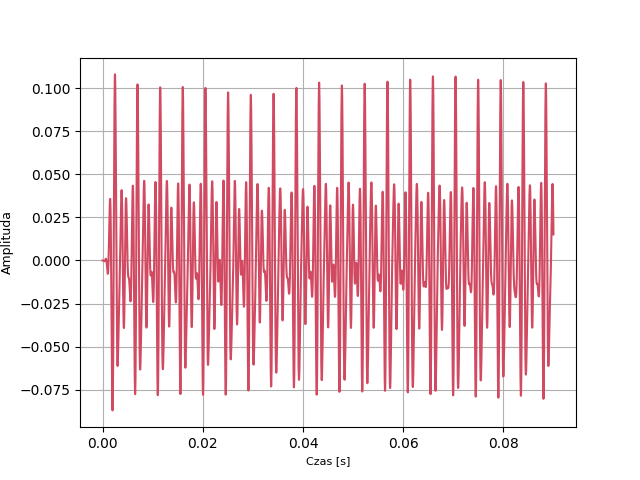
\includegraphics[width=\textwidth]{./img/recordings/HC_a}
        \caption{Sygnał głosu osoby zdrowej (HC)\@}
        \label{fig:recording_HC}
    \end{subfigure}
    \begin{subfigure}{0.49\textwidth}
        \centering
        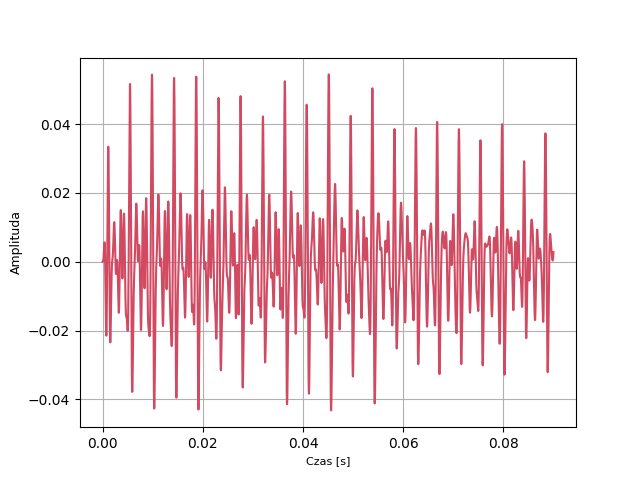
\includegraphics[width=\textwidth]{./img/recordings/PD_a}
        \caption{Sygnał głosu osoby z PD\@}
        \label{fig:recording_PD}
    \end{subfigure}

    \caption{Przykładowe nagrania samogłoski /a/ po preprocessingu (a) dla osoby zdrowej oraz (b) dla osoby z chorobą Parkinsona.}
    \label{fig:recordings}
\end{figure}

\subsection{Obliczanie mel-spektrogramów}
\label{subsec:melspectrogram}

Zdecydowano się na przedstawienie przygotowanych nagrań w formie graficznej w postaci mel-spektrogramów, które zostaną następnie użyte do dalszej analizy.
Spektrogramy to graficzna reprezentacja zmian widma dźwięku w funkcji czasu.
Wykorzystując transformację Fouriera, sygnał dźwiękowy jest podzielony na krótkie ramki czasowe, a następnie dla każdej ramki obliczane jest widmo amplitudowe.
Spektrogram przedstawia te widma w formie kolorowej mapy, gdzie oś pozioma reprezentuje czas, oś pionowa reprezentuje częstotliwość, a intensywność koloru oznacza amplitudę.
Spektrogramy są często wykorzystywane w analizie dźwięku i sygnałów akustycznych.
Pozwalają one zobaczyć, jak zmienia się struktura częstotliwościowa dźwięku w czasie, co może być przydatne do analizy cech akustycznych, identyfikacji dźwięków, diagnostyki medycznej czy rozpoznawania mowy.
Dzięki spektrogramom można wizualnie analizować zmiany w widmie dźwięku, takie jak formanty samogłoskowe, obecność szumów czy artefaktów.

Natomiast mel-spektrogramy to wariant spektrogramów, w których oś częstotliwości jest przekształcona na skalę Mel, czyli nieliniową skalę częstotliwości, która bardziej odpowiada percepcji ludzkiego słuchu.
Stosuje się ją, aby lepiej odzwierciedlić sposób, w jaki odbieramy i rozpoznajemy różnice między różnymi tonami dźwięków.
Przez uwzględnienie charakterystyk percepcji słuchowej człowieka, mel-spektrogramy dostarczają bardziej reprezentatywnych danych akustycznych dla analizy i klasyfikacji dźwięku.
Proces obliczeń mel-spektrogramów został zrealizowany przy użyciu biblioteki języka Python, Librosa.
Wygenerowane mel-spektrogramy zostały przedstawione jako obrazy w skali logarytmicznej (Rys.~\ref{fig:melspectrograms}).

\begin{figure}[ht]
    \centering
    \begin{subfigure}{0.49\textwidth}
        \centering
        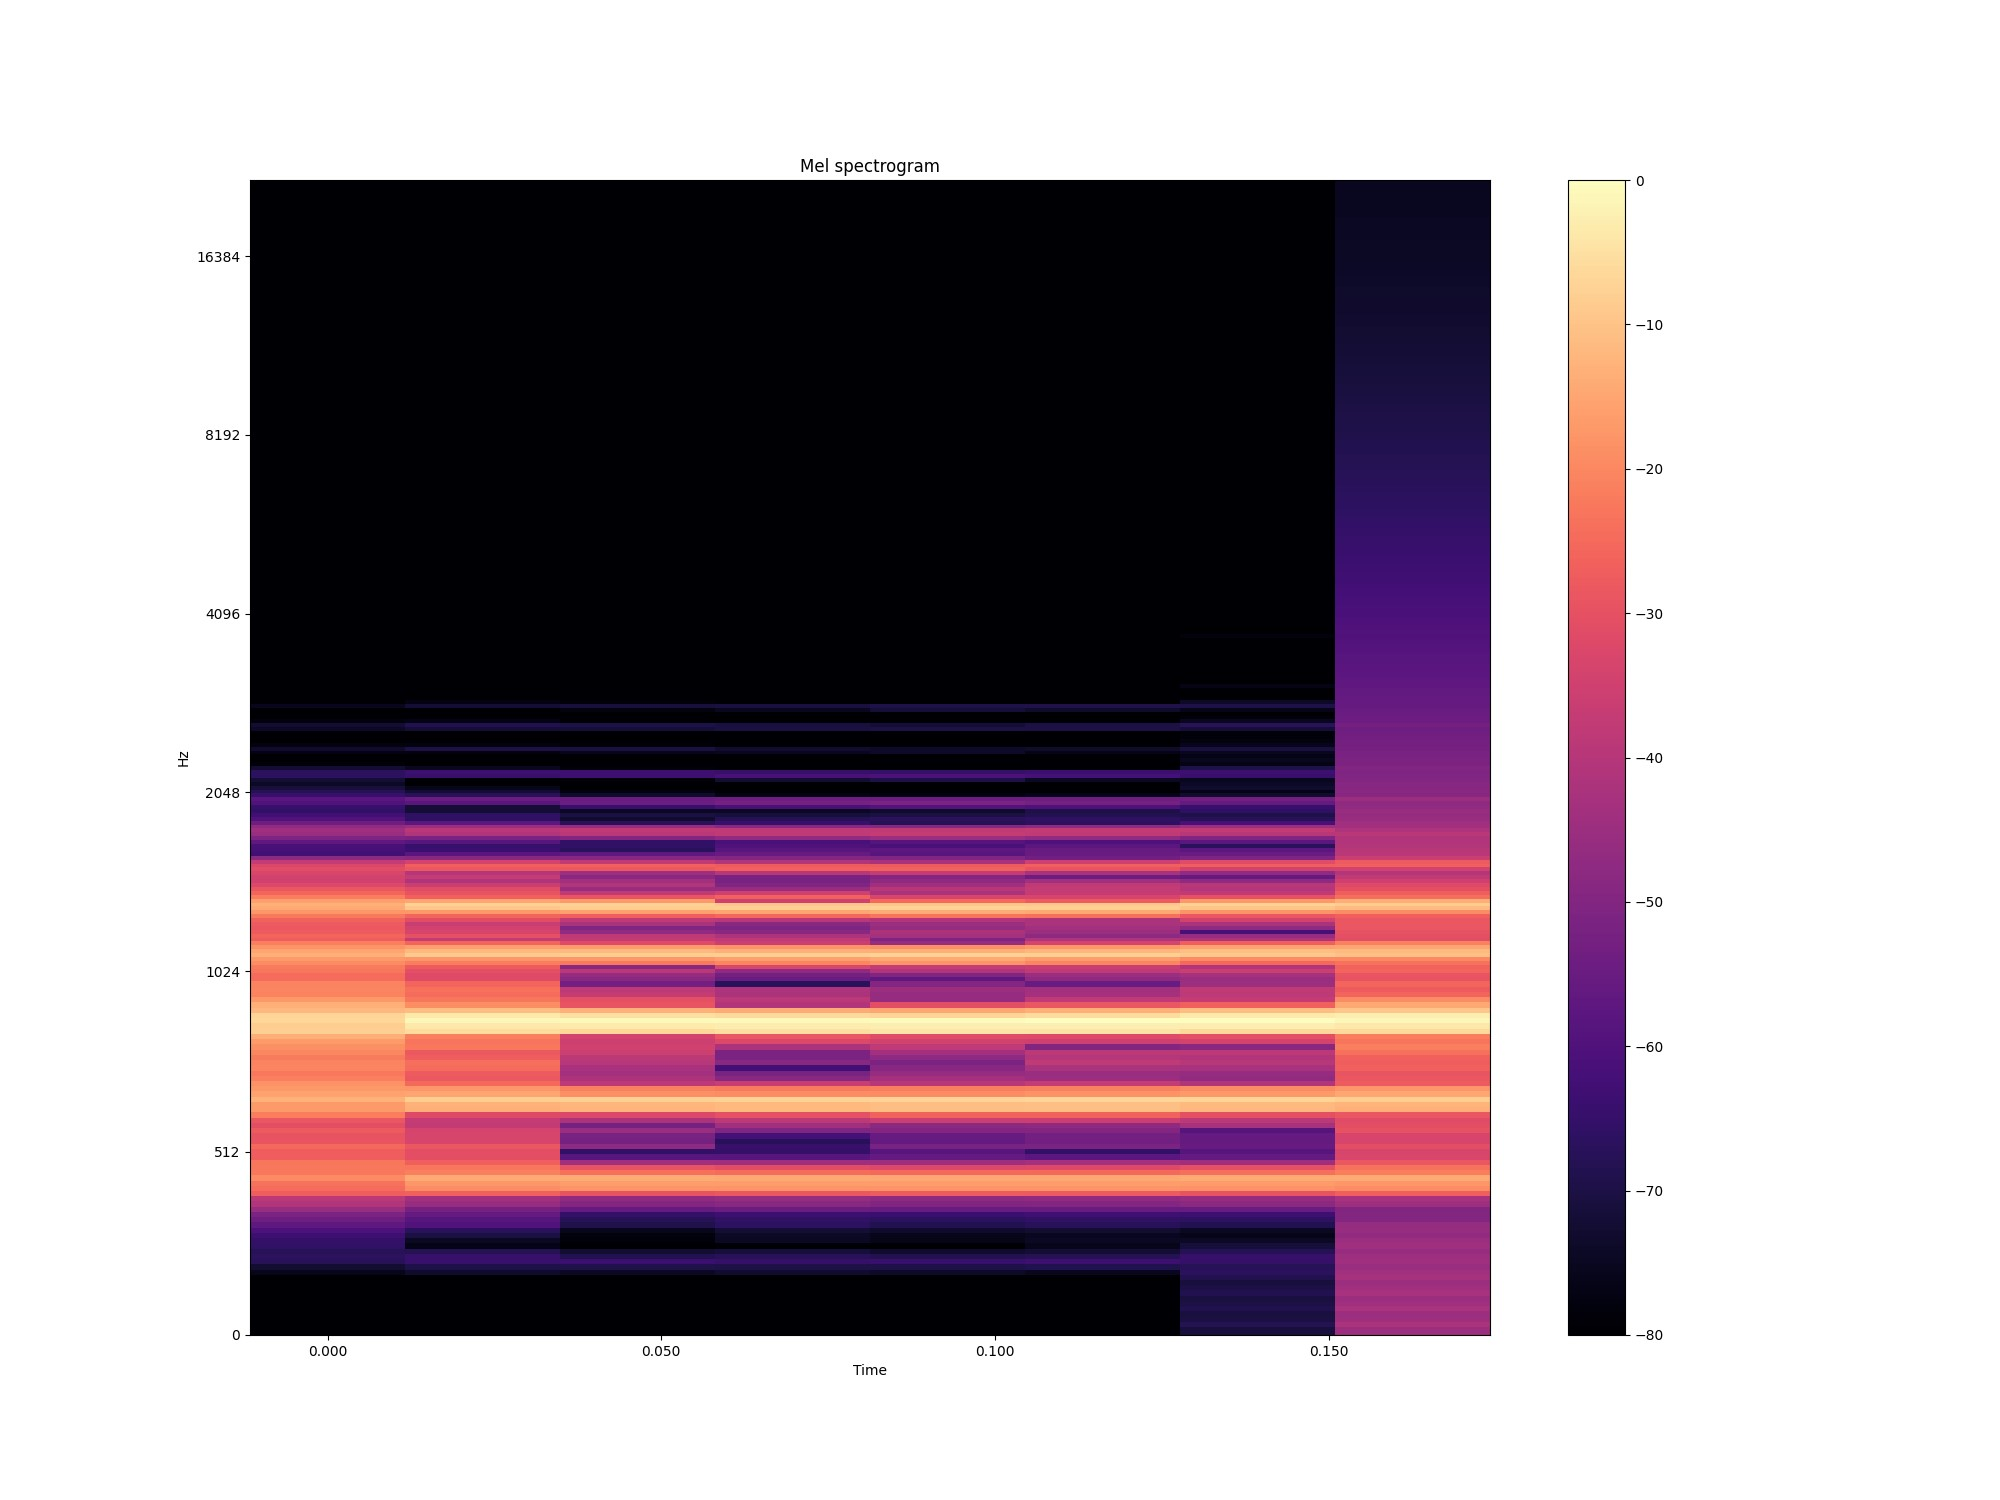
\includegraphics[width=\textwidth]{./img/spectrograms/HC_a}
        \caption{Przykładowy mel-spektrogram dla osoby zdrowej\@}
        \label{fig:melspectrogram_HC}
    \end{subfigure}
    \begin{subfigure}{0.49\textwidth}
        \centering
        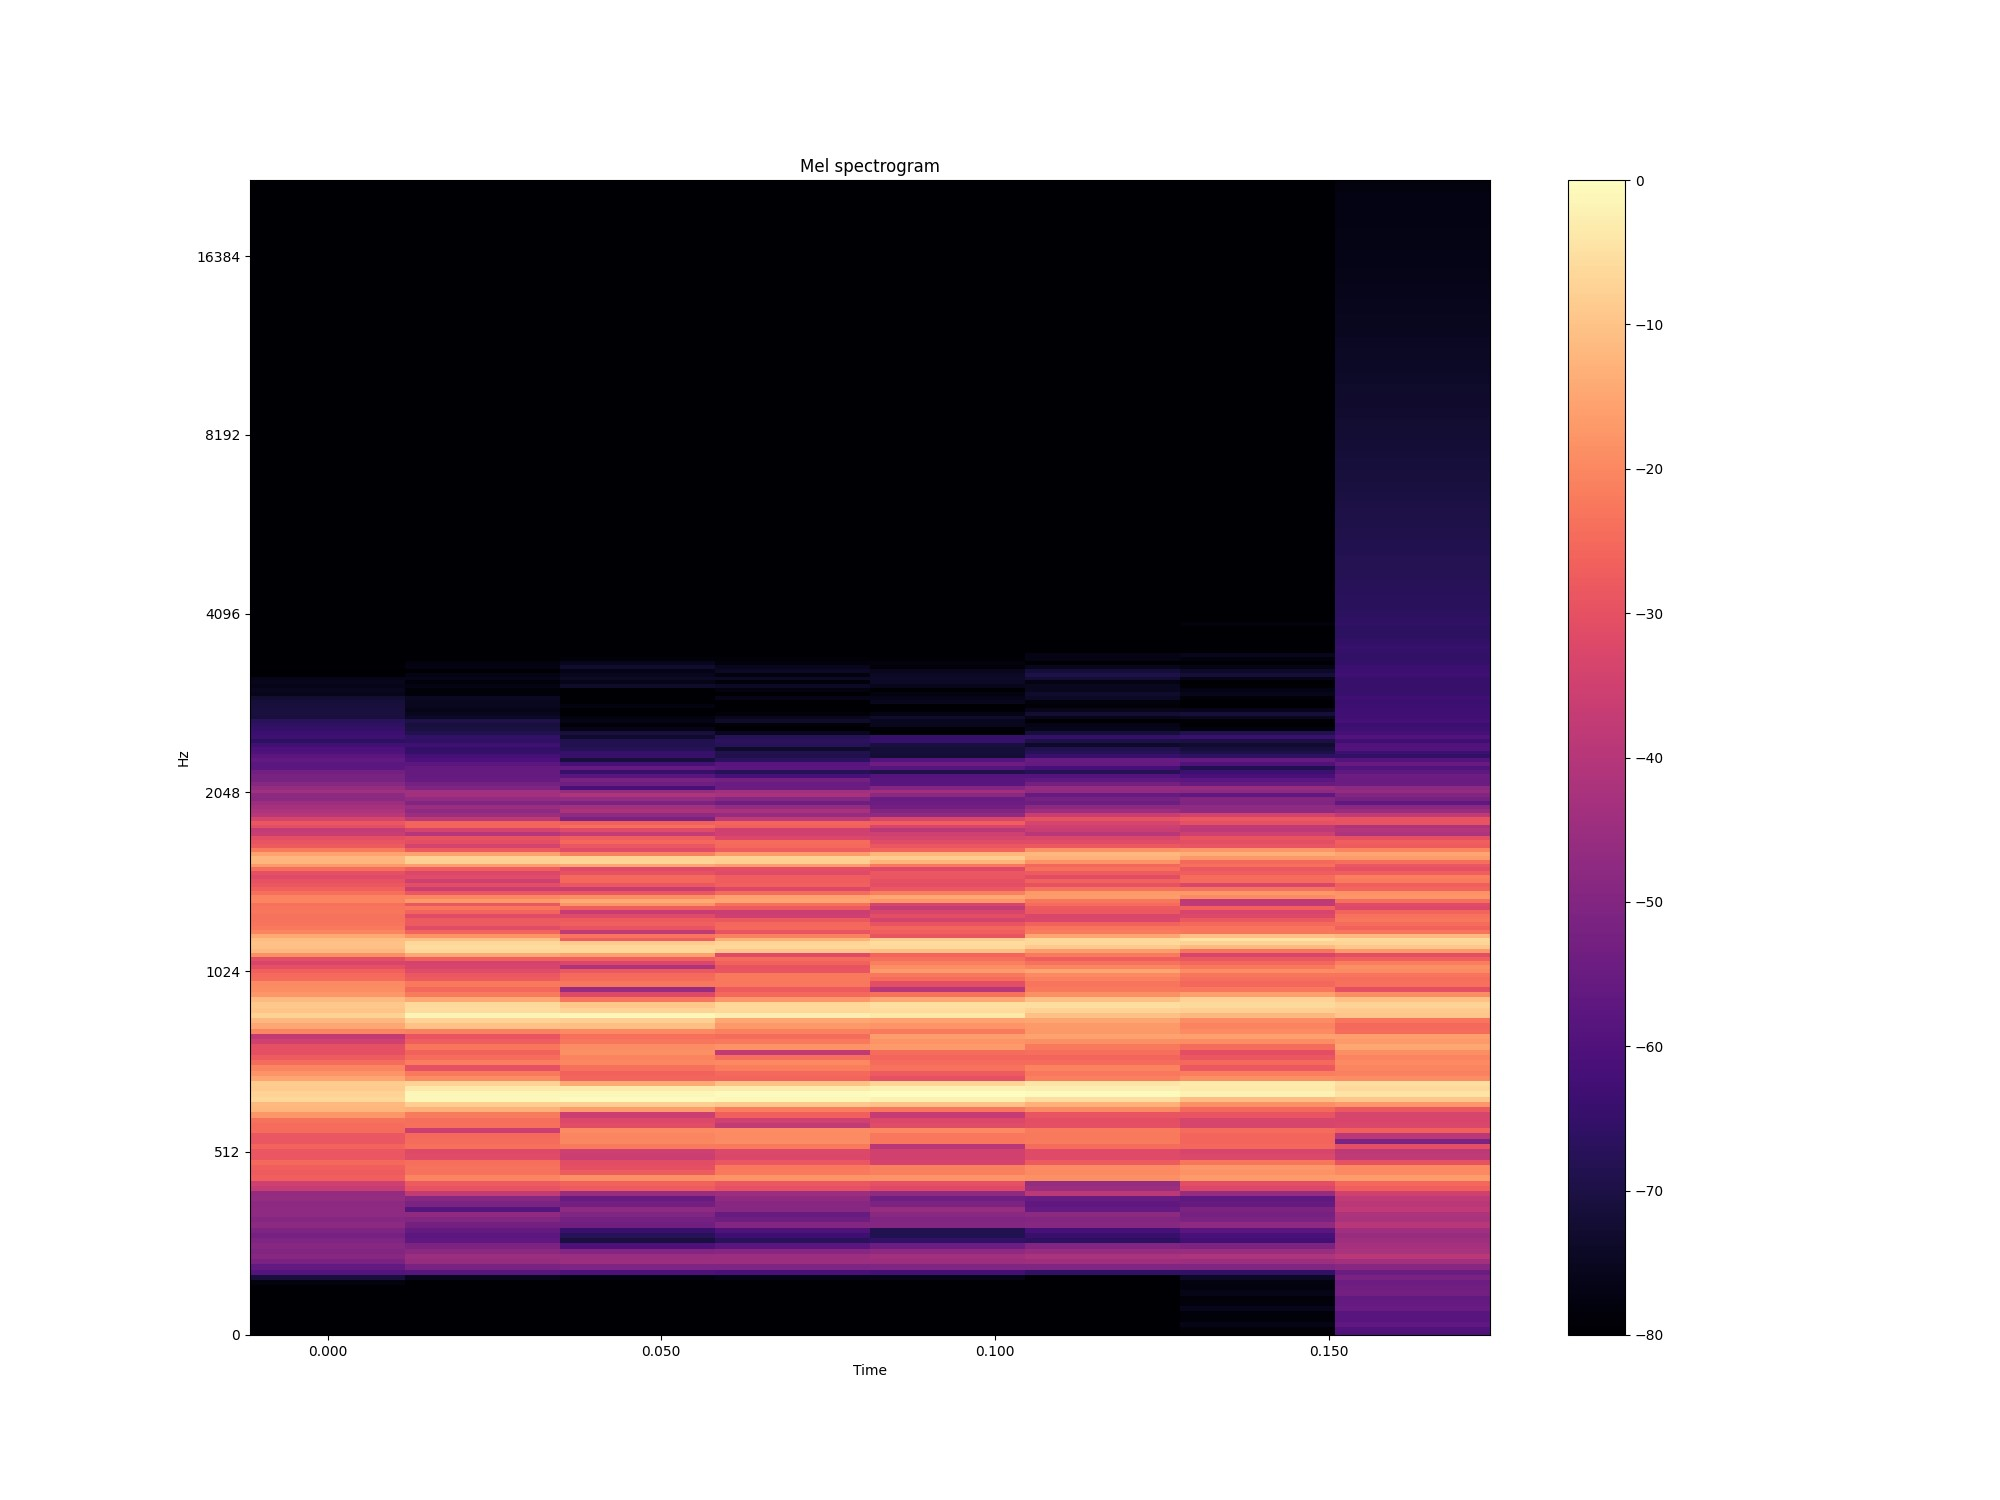
\includegraphics[width=\textwidth]{./img/spectrograms/PD_a}
        \caption{Przykładowy mel-spektrogram dla osoby z PD\@}
        \label{fig:melspectrogram_PD}
    \end{subfigure}

    \caption{Porównanie mel-spektrogramów osoby z PD oraz osoby zdrowej (hiszpańskojęzyczny zbiór danych, samogłoska /a/)}
    \label{fig:melspectrograms}
\end{figure}

Ważnym aspektem przy wyznaczaniu mel-spektrogramów są parametry takie jak liczba pasm Mel, rozmiar ramki analizy, długość przesunięcia (ang. \emph{overlap}) oraz rozdzielczość czasowa i częstotliwościowa.
Różne kombinacje tych parametrów mogą prowadzić do różnych szczegółów w reprezentacji dźwięku.
Wybór tych wartości został przeprowadzony na podstawie dostępną literaturę oraz własne eksperymenty.

Rozmiar okna czasowego jest jednym z kluczowych parametrów obliczeń melspektrogramów.
W kontekście diagnozowania choroby Parkinsona istnieje potrzeba uwzględnienia zarówno krótkotrwałych, dynamicznych zmian w mowie, jak i dłuższych charakterystyk.
Wybór długości okna (2048) został dokonany w celu uzyskania odpowiedniej rozdzielczości w dziedzinie czasu i częstotliwości, co pozwala na dokładniejsze odwzorowanie tych cech w mel-spektrogramie.
Długość przesunięcia określa, co ile próbek dźwiękowych nowe okno czasowe jest nakładane na sygnał.
W celu zachowania równowagi między dokładnością w dziedzinie czasu a efektywnością obliczeń wybrano \emph{hop\_length} o wartości 512.
Jest to kompromis, który pozwala na zachowanie informacji o krótkotrwałych zmianach w sygnale.
Liczba pasm Mel określa, ile pasm częstotliwościowych zostanie wygenerowanych w mel-spektrogramie.
W celu uzyskania szczegółowej reprezentacji widma dźwiękowego wybrano wartość równą 320.
Choroba Parkinsona może wprowadzać subtelne zmiany w mowie, dlatego ważne jest uwzględnienie wysokiej rozdzielczości w dziedzinie częstotliwości, co pozwala na dokładniejszą analizę sygnału mowy.


Często praktyką przed przekazaniem danych do sieci neuronowych (CNN) jest ich skalowanie.
Pomaga ono zapewnić zbieżność, stabilność i efektywność procesu uczenia się modelu, nie wprowadzając dodatkowych informacji.
Dlatego zdecydowano się na skalowanie metodą \emph{Min-Max}  na zakres od 0 do 1 opisaną wzorem~\eqref{eq:minmax}.

\begin{equation}
	\label{eq:minmax}
	X_{\text{scaled}} = \frac{X - X_{\min}}{X_{\max} - X_{\min}}
\end{equation}

\subsection{Augmentacja}
\label{subsec:augmentacja}

Aktualny stan wiedzy w dziedzinie automatycznej diagnostyki choroby Parkinsona ukazuje, że konwolucyjne sieci neuronowe (CNN) znacząco poprawiły wyniki w zadaniach przetwarzania mowy.
Jednakże, aby uniknąć przeuczenia, konieczna jest duża ilość danych treningowych.
Dostępne bazy danych zawierają zwykle do kilkuset nagrań, co ogranicza możliwość uwzględnienia wielu istotnych cech i stworzenia stabilnego modelu klasyfikacyjnego.

W początkowych eksperymentach przeprowadzonych w ramach tej pracy nie udało się osiągnąć oczekiwanych wyników, ze względu na bardzo duże przeuczenie (ang. \emph{overfitting}) testowanych modeli.
Jest to częsty problem, który można rozwiązać dzięki praktyce znanej jako augmentacja danych.
Polega ona na modyfikacji oryginalnych próbek, co prowadzi do zwiększenia ilości danych treningowych.
Augmentacja danych znacząco poprawia zdolność modeli CNN do generalizacji i zwiększa ich odporność na przeuczenie.

W badaniu opisanym w publikacji~\cite{augmentation} zastosowano sześć technik augmentacji danych specyficznych dla mowy w celu polepszenia zdolności modelu do generalizacji na dane, które nie były wcześniej widziane.
Wyniki tych badań pokazały, że wykorzystane techniki augmentacji  istotnie poprawiały zdolność do wykrywania zaburzeń mowy u pacjentów z chorobą Parkinsona.
Podobne znaczenie augmentacji danych jako istotnego czynnika wpływającego na skuteczność rozwiązań w dziedzinie klasyfikacji choroby Parkinsona podkreślono również w publikacji~\cite{Wodzinski}.

Dlatego w niniejszej pracy zdecydowano się zastosować 4 techniki augmentacyjne: przesunięcie w czasie, spowolnienie, przyspieszenie oraz losową zmianę wysokości dźwięku.
Wszystkie modyfikacje zostały przeprowadzone na sygnałach przed wyznaczeniem mel-spektrogramów.
Wpływ zmian na mel-spektrogramy przedstawiono na Rys~\ref{fig:augumentacja}.


\begin{enumerate}[label={\alph*)}]
	\item Przesunięcie w czasie (ang.~\emph{time shifting}). Dla zapewnienia, że model nie dostosowuje się do lokalizacji czasowej danej próbki mowy lub głosu, zmieniana jest kolejność sygnału.
Jest to osiągane poprzez przesunięcie sygnałów w prawo wzdłuż osi czasu o losową ilość, która jest mniejsza niż długość wejściowego nagrania audio.
    \item Losowa zmiana wysokości dźwięku (ang.~\emph{pitch change}). Składowe częstotliwości próbek są losowo przesuwane w dół lub w górę, przy czym należy zadbać o to, aby długość nie uległa zmianie poprzez rozciągnięcie oryginalnej próbki o losową ilość czasu z przedziału [3; 5] w dziedzinie czasu, a następnie jej resampling.
    \item Spowolnienie (ang.~\emph{slow-down}).
Przez rozciągnięcie w czasie próbki dźwiękowej zapewniamy, że model sieci neuronowej nie dostosowuje się tylko do prędkości mowy lub głosu badanego podmiotu.
Współczynnik spowolnienia jest losowo wybierany z przedziału [0,2; 0,8].
    \item Przyspieszenie (ang.~\emph{speed-up}). Tak samo, jak spowolnienie dźwięku, losowe przyspieszenie ma na celu zapobieganie dostosowywaniu modelu do prędkości mowy mówcy.
Współczynnik przyspieszenia jest losowo wybierany z przedziału [1,2; 2,5].
\end{enumerate}

Augmentacja została przeprowadzona tylko dla zbioru treningowego i walidacyjnego, aby zwiększyć różnorodność danych uczących oraz poprawić wydajność modelu w procesie uczenia maszynowego.
Zbiór testowy pozostaje nienaruszony, aby zachować jego niezmienność i umożliwić obiektywną ocenę skuteczności modelu na nieznanych wcześniej danych.

\begin{figure}[hp]
    \centering
    \begin{subfigure}{0.68\textwidth}
        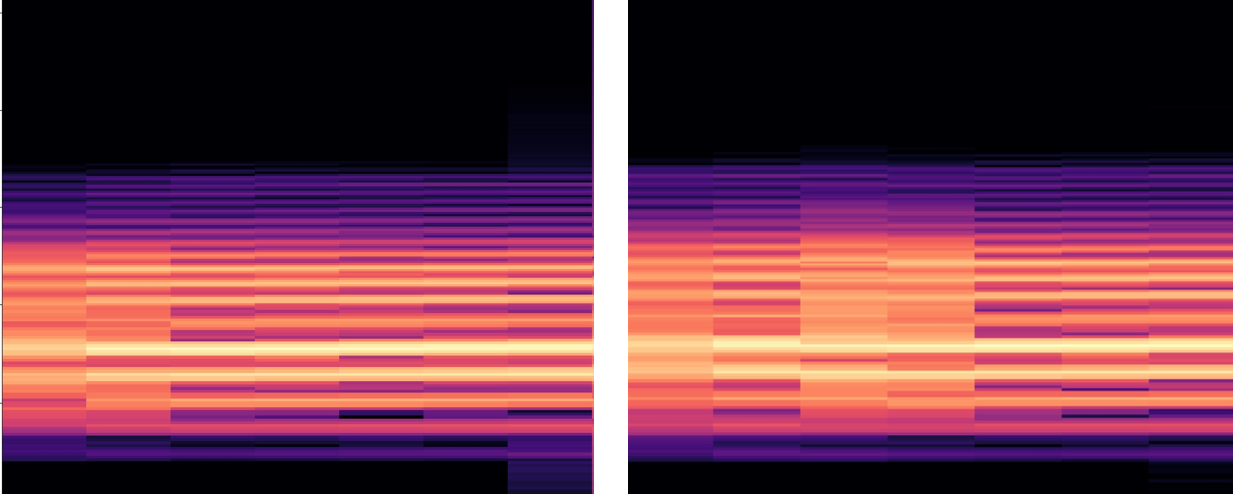
\includegraphics[width=\linewidth]{./img/augmentation/rolled}
        \caption{Przesunięcie w czasie\@}
        \label{fig:roll}
    \end{subfigure}

    \begin{subfigure}{0.68\textwidth}
        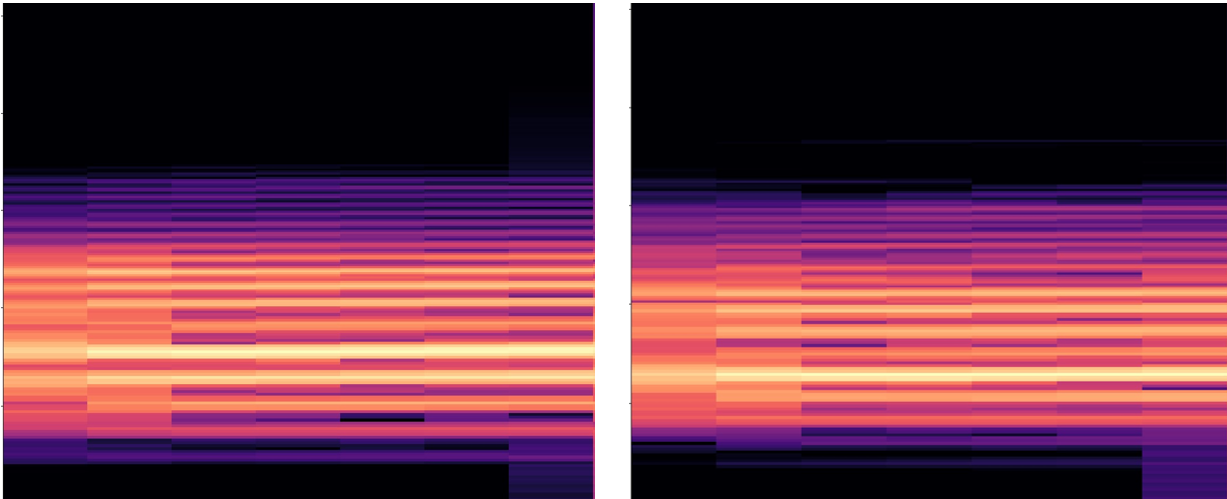
\includegraphics[width=\linewidth]{./img/augmentation/pitch}
        \caption{Zmiana wysokości dźwięku\@}
        \label{fig:pitch}
    \end{subfigure}

    \begin{subfigure}{0.68\textwidth}
        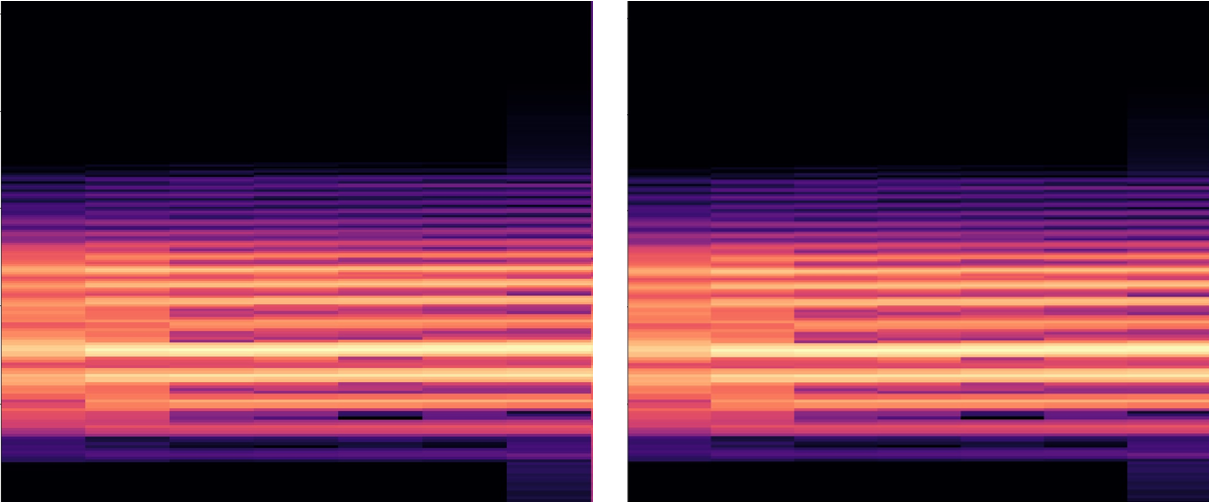
\includegraphics[width=\linewidth]{./img/augmentation/slow}
        \caption{Spowolnienie\@}
        \label{fig:slow}
    \end{subfigure}

    \begin{subfigure}{0.68\textwidth}
        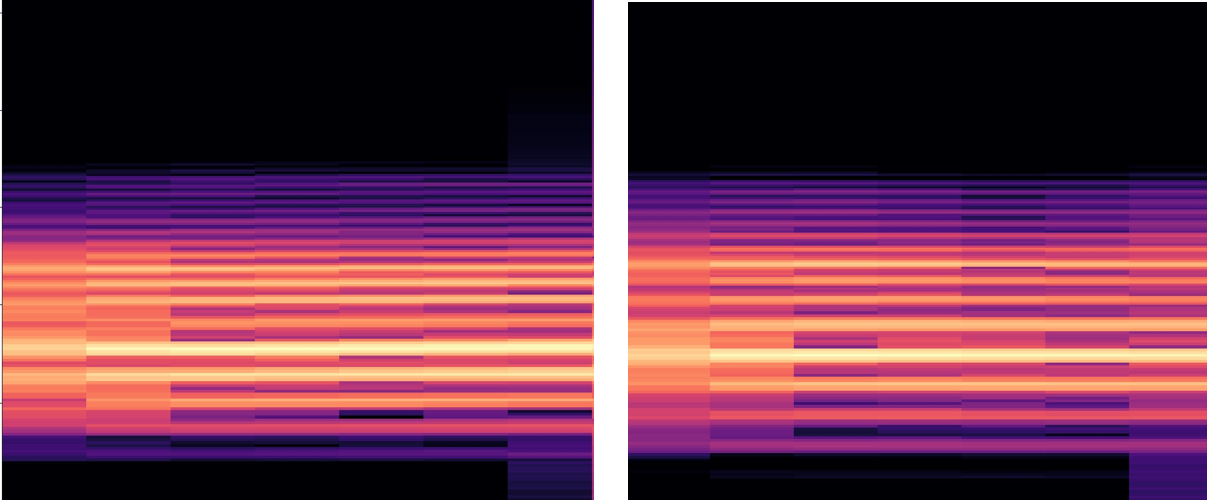
\includegraphics[width=\linewidth]{./img/augmentation/speed}
        \caption{Przyspieszenie\@}
        \label{fig:speed}
    \end{subfigure}

    \caption{Porównanie wpływu technik augmentacji na wygląd mel-spektrogramu. Po lewej stronie przedstawiony jest mel-spektrogram obliczony na podstawie surowego sygnału, a po prawej stronie widoczne są efekty augmentacji, w kolejności: (a) przesunięcie w czasie, (b) zmiana wysokości dźwięku, (c) spowolnienie sygnału oraz (d) przyspieszenie sygnału. (Zbiór danych: PC-GITA, samogłoska /a/, HC)}

    \label{fig:augumentacja}
\end{figure}

%---------------------------------------------------------------------------
%\newpage
\section{Metody klasyfikacji}
\label{sec:klasyfikacja}

Zdecydowano się na graficzne reprezentacje sygnałów, co wymaga też doboru odpowiednich metod klasyfikacji.
Popularnym rozwiązaniem są konwolucyjne sieci neuronowe (ang. \emph{Convolutional Neural Network}, CNN).
Jest to rodzaj zaawansowanych modeli uczenia maszynowego, które zostały pierwotnie zaprojektowane do przetwarzania i analizy danych wizualnych, takich jak obrazy i filmy.
Jednakże, ze względu na swoją skuteczność w ekstrakcji cech z danych przestrzennych, CNN znalazły zastosowanie także w dziedzinach związanych z przetwarzaniem dźwięku.

Główną cechą CNN są warstwy konwolucyjne.
Wykorzystują one filtry konwolucyjne, które przesuwają się po wejściowych danych, wyodrębniając lokalne wzorce, takie jak krawędzie, tekstury i inne cechy.
To pozwala na automatyczną ekstrakcję istotnych cech.
CNN często zawierają też warstwy \emph{pooling}, które zmniejszają rozmiar danych wyjściowych z warstw konwolucyjnych.
Pomaga to zmniejszyć liczbę parametrów w sieci i sprawia, że sieć jest bardziej odporna na przetwarzanie danych o różnych rozmiarach.
CNN zwykle składają się z wielu warstw konwolucyjnych i warstw \emph{fully connected}, które uczą się reprezentacji coraz bardziej abstrakcyjnych cech danych.
Są wysoce zdolne do rozpoznawania wzorców w danych, co czyni je skutecznymi w zadaniach klasyfikacji, detekcji obiektów, rozpoznawaniu mowy i wielu innych.
Dużą zaletą sieci konwolucyjnych jest możliwość skorzystania z uczenia z transferem, co oznacza wykorzystanie pretrenowanych modeli na dużych zbiorach danych, a następnie dostosowanie ich do konkretnej dziedziny lub zadania.

Konwolucyjne sieci neuronowe są potężnym narzędziem w analizie graficznych reprezentacji danych i są powszechnie stosowane w wielu dziedzinach, aby automatycznie ekstrahować i analizować cechy złożonych danych przestrzennych.
Dzięki ich zdolności do hierarchicznego uczenia się i rozpoznawania wzorców są używane w różnych zastosowaniach, w tym również w medycynie.
Dlatego zdecydowano się wykorzystać tę metodę do klasyfikacji mel-spektrogramów.

\subsection{Wykorzystane architektury}
\label{subsec:architektury}

Ze względu na ograniczoną dostępność danych głosowych pacjentów z chorobą Parkinsona, zastosowano technikę znaną jako \emph{transfer learning}.
Umożliwia ona wykorzystanie wstępnie wytrenowanych modeli, które zostały nauczane na dużym zbiorze danych,
do zadań diagnostycznych z wykorzystaniem ograniczonej ilości dostępnych danych głosowych.

Kluczowym krokiem było wybranie modeli, które miały dostępne wagi wytrenowane na dużym i takim samym zbiorze danych.
Zdecydowano się na ImageNet, ponieważ jest to jedna z najważniejszych baz danych obrazów wykorzystywana w dziedzinie komputerowego widzenia i uczenia maszynowego.
Wybrano modele takie jak Xception, MobileNetV2, InceptionV3, VGG16 i ResNet50.
Takie podejście pozwoliło na zaoszczędzenie czasu i zasobów, które byłyby potrzebne do wytrenowania sieci od podstaw na niewielkim zbiorze danych.
W ramach pracy magisterskiej skoncentrowano się na porównaniu różnych architektur w kontekście automatycznej diagnostyki choroby Parkinsona na podstawie analizy głosu.

\begin{enumerate}[label={\alph*)}]
    \item VGG16. To przykład klasycznego modelu CNN o głębokiej architekturze, opracowany przez Visual Geometry Group na Uniwersytecie Oksfordzkim.
    Jest znany ze swojej prostoty i skuteczności w ekstrakcji cech z obrazów.

    \item ResNet50. Jest to znana architektura CNN, która wprowadza innowacyjny pomysł na połączenia pomostowe, eliminujące problem znikającego gradientu w głębokich sieciach.
    Dzięki temu ResNet50 jest w stanie efektywnie uczyć się reprezentacji danych.

    \item Xception. Jest to model głębokiej nauki opracowany przez François Chollet w 2016 roku.
    Jest to jedna z odmian architektury konwolucyjnej sieci neuronowej (CNN), która wyróżnia się wyjątkową zdolnością do wykrywania cech hierarchicznych w obrazach.

    \item InceptionV3. Charakteryzuje się wykorzystaniem tzw. \emph{inception modules}, które pozwalają na efektywne wykrywanie wielu skal i rodzajów cech w obrazach.
    Został zaprojektowany przez Google.

    \item MobileNetV2. Jest to przykłąd lekkiej i efektywnej architektury CNN, zaprojektowanej z myślą o urządzeniach mobilnych
    Jej cechą charakterystyczną jest niska ilość parametrów i małe obliczenia, co sprawia, że jest idealna do zastosowań w zasobochłonnych zadaniach takich jak analiza głosu na urządzeniach mobilnych.

\end{enumerate}

Wybór tych konkretnych klasyfikatorów wynikał z różnorodności ich architektur i specjalizacji.
Choroba Parkinsona manifestuje się na różne sposoby w głosie pacjentów, dlatego zróżnicowane modele w różny sposób mogą wspomagać wydobycie istotnych cech.
Xception i InceptionV3 są znane z efektywności w ekstrakcji wielu rodzajów cech, co jest istotne przy analizie złożonych danych głosowych.
MobileNetV2, z kolei, jest lekki i mobilny, co pozwala na przenośność rozwiązania do urządzeń mobilnych, które mogą być używane w codziennym monitoringu pacjentów.
VGG16 i ResNet50, choć głębokie, mają zdolność do wyodrębniania skomplikowanych wzorców, co może być przydatne w diagnozie.
Porównanie różnych klasyfikatorów pozwoli na ocenę ich wydajności i skuteczności w diagnostyce na podstawie głosu.

Po początkowym przeszkoleniu na zbiorze danych ImageNet przeprowadzono proces \emph{fine-tuningu} na wcześniej przygotowanym zestawie danych.
Fine-tuning to technika dostosowywania już przeszkolonych modeli do specyficznych zastosowań.
Modele były dostosowywane w celu nauki rozpoznawania specyficznych cech akustycznych charakterystycznych dla pacjentów z chorobą Parkinsona.
Proces ten obejmował dodawanie dodatkowych warstw gęstych do modelu oraz wykorzystywanie techniki dropout, która pomaga uniknąć przeuczenia modelu.
Dzięki tym modyfikacjom klasyfikatory stały się bardziej odpowiednie do analizy dźwięku oraz diagnozowania choroby Parkinsona na podstawie danych głosowych

%W każdym przypadku wykorzystano pretrenowane wagi do ekstrakcji cech.
%Ostatnią warstwę gęstą zastąpiono odpowiednimi warstwami, zależnie od architektury sieci.
%Konfiguracje te zostały dobrane na podstawie zarówno dostępnej literatury, jak i własnych eksperymentów.

%W przypadku sieci VGG16  i InceptionV3 dodano jedną warstwę \emph{Dense} o rozmiarze 512 oraz warstwę Dropout o współczynniku 0,5.
%W ResNet50 oraz dodano warstwę dense o rozmiarze 128.
%W przypadku Xception podobnie jak w publikacji~\cite{augmentation}, dodano trzy warstwy dense o rozmiarze 128 oraz warstwę Dropout o współczynniku 0,5.
%W sieci MobileNetV2 dodano dwie warstwy dense o rozmiarze 128 oraz warstwę Dropout o współczynniku 0,5.
%Na koniec, do każdej z tych architektur dodaliśmy warstwę gęstą z dwoma neuronami i funkcją aktywacji~\emph{softmax}), aby umożliwić skuteczną klasyfikację.

\subsection{Dobór parametrów i optymalizacja modeli}
\label{subsec:optymalizacja-modeli}

Wszystkie eksperymenty przeprowadzono przy użyciu tych samych parametrów.
Testowano różne kombinacje, jednak te ustawienia okazały się optymalne dla badanego problemu.
W eksperymentach uwzględniono takie aspekty jak rozmiar partii (ang. \emph{batch-size}), funkcję  straty i optymalizator.

Wybór rozmiaru partii, czyli liczby próbek przetwarzanych jednocześnie przez sieć neuronową, ma znaczenie dla równowagi pomiędzy wydajnością obliczeniową a stabilnością procesu  uczenia.
Przyjęto rozmiar partii równy 32, co jest kompromisem między efektywnym wykorzystaniem zasobów obliczeniowych a stabilnością uczenia.

Funkcja straty, czyli binarna entropia krzyżowa, została wybrana ze względu na swoją skuteczność w problemach klasyfikacji binarnej.
Minimalizacja funkcji straty pozwala modelowi lepiej dopasować się do rzeczywistych klas i ocenić jakość predykcji sieci.
Ta metryka jest często stosowana w zadaniach klasyfikacji, ponieważ skupia się na porównywaniu prognozowanych klas z rzeczywistymi wartościami.

Wybór optymalizatora SGD (ang. \emph{Stochastic Gradient Descent}) był wynikiem eksperymentalnej analizy różnych algorytmów optymalizacji i ich właściwości.
Ponadto jest on najczęściej spotykany w literaturze dotyczącej tego problemu badawczego.
W każdej iteracji SGD losowo wybiera małe losowe podzbiory danych treningowych i oblicza gradient funkcji kosztu tylko na podstawie tych próbek, co pozwala na szybszą aktualizację wag modelu.
Ta stochastyczna natura SGD pomaga uniknąć utknięcia w minimach lokalnych.

Bardzo ważny w tym problemie klasyfikacyjnym jest odpowiedni dobór współczynnika uczenia (ang. \emph{learning rate}).
Wartość tego parametru wpływa na tempo, z jakim model aktualizuje swoje wagi podczas procesu uczenia.
Wysoki learning rate może prowadzić do oscylacji i trudności w zbieżności algorytmu, podczas gdy zbyt niski może spowolnić proces uczenia.
Dlatego optymalny wybór \emph{learning rate} jest istotnym krokiem w dostrojeniu algorytmu SGD do konkretnego problemu.
Zdecydowano się na ustawienie wartości współczynnika uczenia na 0,0005.

Modele były trenowane przez 50 epok, ponieważ zbyt duża liczba epok mogłaby prowadzić do przetrenowania na tak małej ilości danych, co wpłynęłoby negatywnie na ich zdolność do generalizacji na nowe dane.
Dodatkowo zastosowano monitorowanie funkcji straty.
Ten mechanizm umożliwia wczesne zatrzymanie treningu, jeśli funkcja straty przestaje się poprawiać przez określoną liczbę epok (w tym przypadku przyjęto 5).

\subsection{Podział danych}
\label{subsec:podzial-danych}

Klasyczną techniką w uczeniu maszynowym jest podział zbioru danych na 3 podzbiory: treningowy, testowy oraz walidacyjny.
W problemie klasyfikacji celem jest stworzenie algorytmu, który na podstawie znanych sobie, opisanych wzorców, będzie w stanie efektywnie rozpoznawać wzorce nieopisane i dotąd sobie nieznane.
Dlatego wydziela się zbiór treningowy, na podstawie którego model uczy się wzorców i dopasowuje do danych.
Aby uniknąć nadmiernego dopasowania danych do modelu (ang.
\emph{overfitting}) stosuje się również zbiór walidacyjny, który  przeprowadza bezstronną ocenę dopasowania modelu do zbioru danych szkoleniowych podczas dostrajania hiperparametrów modelu.
Na koniec ocenia się skuteczność modelu na niezależnym zbiorze testowym.

Inną często wykorzystywaną techniką jest wykorzystanie krosswalidacji (ang. \emph{cross-validation}).
Jest to technika oceny wydajności modelu maszynowego, która polega na podziale dostępnych danych na kilka części, z których jedna służy jako zbiór walidacyjny, a pozostałe jako zbiór treningowy.
Proces ten jest wielokrotnie powtarzany, aby uzyskać stabilniejszą ocenę wydajności modelu i uniknąć przeuczenia.
Najpopularniejszym typem krosswalidacji jest walidacja krzyżowa typu k-fold, gdzie dane są dzielone na k podzbiorów, a każdy z nich jest używany jako zbiór testowy w jednym z k cykli walidacji.

W pracy zastosowano 10-krotną walidację krzyżową oraz przyjęto podział na zbiór treningowy i testowy według proporcji 80:20 (biorąc pod uwagę osoby, nie liczbę nagrań).
Ważnym aspektem jest fakt, że podział nagrań dla różnych samogłosek przeprowadzono biorąc pod uwagę tożsamość mówcy (podejście \emph{subject-wise}).
To znaczy, że na przykład nagrania osoby, która znajduje się w zbiorze treningowym nie mogą wystąpić ani w testowym, ani walidacyjnym.
Ta zasada obowiązuje we wszystkich podzbiorach.
Pomaga to zachować spójne warunki uczenia i obiektywnie porównać otrzymane modele.
Nie dopuszcza to też możliwości, że model uczy się wzorców związanych z osobą, a nie chorobą Parkinsona.
Ostatecznie w zbiorze testowym znalazło się 90 nagrań od 30 osób.
W zbiorach walidacyjnym i treningowym liczby te nieco różniły się w różnych iteracjach krosswalidacji, ponieważ nie dla każdego mówcy dysponowano taką samą ilością nagrań.
Zbiór walidacyjny zawierał około 45 nagrań, a treningowy około 350.

%---------------------------------------------------------------------------

\section{Metody ewaluacji wyników}
\label{sec:metody-ewaluacji-wynikow}

W celu oceny skuteczności różnych metod klasyfikacji choroby Parkinsona przeprowadzono badania wykorzystujące różnorodne techniki ewaluacji.
Niniejsza sekcja zawiera prezentację wybranych metod, które zostały użyte w ramach przeprowadzonych eksperymentów.
Kluczowym aspektem jest konieczność zastosowania odpowiednich technik ewaluacji wyników.
Techniki te nie tylko umożliwiają obiektywną ocenę efektywności proponowanych rozwiązań, ale także pozwalają na porównanie ich ze sobą.
Dzięki temu pozwalają lepiej zrozumieć, które podejścia są najbardziej obiecujące w kontekście diagnozowania choroby Parkinsona i polepszania dokładności klasyfikacji, co jest kluczowe dla postępu w dziedzinie medycyny i diagnostyki tej choroby.

\subsection{Krzywe uczenia}
\label{subsec:krzywe-uczenia}

Krzywe uczenia są skutecznym narzędziem do wizualizacji procesu uczenia modelu.
W trakcie eksperymentów prowadzono monitorowanie dwóch kluczowych krzywych: dokładność (ang. \emph{accuracy}) i funkcję kosztu (ang. \emph{loss}).
Krzywa dokładności przedstawia zmiany dokładności modelu w trakcie treningu i walidacji, podczas gdy krzywa funkcji kosztu pokazuje, jak zmienia się funkcja kosztu w trakcie uczenia.
Analiza tych krzywych dostarcza istotnych informacji na temat efektywności uczenia modelu.
Pozwala ocenić, czy model uczy się poprawnie, czy może występują problemy z nadmiernym dopasowaniem  (ang. \emph{overfitting}) lub niedostatecznym dopasowaniem (ang. \emph{underfitting}).
Dzięki tym analizom można dokonać wniosków na temat jakości modelu i ewentualnie dostosować hiperparametry lub strategię treningową w celu uzyskania lepszych wyników.
Wartościowe informacje o procesie uczenia są kluczowe dla udanej implementacji modelu i oceny jego skuteczności.

\subsection{Metryki walidacyjne}
\label{subsec:metryki-waldiacyjne}

Podczas oceny skuteczności klasyfikacji, korzystano z najbardziej popularnych metryk, które pozwalają ocenić jakość predykcji modelu.
W podanych wzorach zastosowano oznaczenia:  TP – True Positive, TN – True Negative, FP – False Positive, FN – False Negative.

\begin{enumerate}[label={\alph*)}]
    \item Błędy I i II rodzaju
    \item [] Jest to popularne narzędzie służące do analizy wyników klasyfikacji.
    Błąd I rodzaju (ang. \emph{False Positive}) oznacza błędną klasyfikację przypadku, który jest negatywny, jako pozytywny.
    W kontekście Parkinsona oznacza to, że model zaklasyfikował zdrową osobę jako chorą na chorobę Parkinsona.
    Błąd II rodzaju (ang. \emph{False Negative}) oznacza błędną klasyfikację przypadku, który jest pozytywny, jako negatywny.
    W kontekście Parkinsona oznacza to, że model zaklasyfikował osobę chorą na chorobę Parkinsona jako zdrową.

    \item [] Analiza błędów I i II rodzaju ma duże znaczenie w kontekście ewaluacji systemów diagnostycznych.
    Błąd I rzędu może prowadzić do niezdiagnozowania choroby u pacjenta, podczas gdy błąd II rzędu może prowadzić do błędnego zdiagnozowania osoby zdrowej jako cierpiącej na chorobę Parkinsona.
    Ważne jest, aby oceniać i minimalizować te błędy w celu uzyskania jak najdokładniejszej klasyfikacji.

    \item [] W systemach diagnostycznych większe znaczenie ma minimalizacja błędów II rodzaju.
    W przypadku wykorzystania takiego narzędzia jako wspomagającego proces diagnozy zaklasyfikowanie osoby zdrowej jako chorej spowoduje jedynie dalszą diagnostykę.
    Natomiast jeśli osoba chora rozpoznana zostanie jako zdrowa, proces jej leczenia rozpocznie się później, co może przynieść różne skutki.
	\item Dokładność (ang.~\emph{accuracy})
    \item [] To prosta i intuicyjna miara, która oblicza stosunek poprawnie sklasyfikowanych próbek do wszystkich próbek.
    Wyraża ona ogólną skuteczność klasyfikacji.
    Opisywana jest wzorem~\ref{eq:accuracy}
    \begin{equation}
        \text{Accuracy} = \frac{TP + TN}{TP + FN + TN + FP}
        \label{eq:accuracy}
    \end{equation}
    , gdzie:

\quad$TP$ - True Positives (prawdziwie pozytywne),

\quad$TN$ - True Negatives (prawdziwie negatywne),

\quad$FP$ - False Positives (fałszywie pozytywne),

\quad$FN$ - False Negatives (fałszywie negatywne).

    \item Precyzja (ang.~\emph{precision})
    \item [] Mierzy stosunek prawdziwie pozytywnych predykcji do sumy prawdziwie pozytywnych i  fałszywie pozytywnych predykcji.
Wyraża zdolność modelu do identyfikowania prawdziwie pozytywnych przypadków.
Określa się ją wzorem~\ref{eq:precision}
      \begin{equation}
        \text{Precision} = \frac{TP}{TP + FP}\label{eq:precision}
    \end{equation}
    , gdzie:

\quad$TP$ - True Positives (prawdziwie pozytywne),

\quad$FP$ - False Positives (fałszywie pozytywne).

    \item Czułość (ang.~\emph{recall})
    \item [] Jest to stosunek prawdziwie pozytywnych predykcji do sumy prawdziwie pozytywnych i fałszywie negatywnych predykcji.
Wyrażana jest wzorem~\ref{eq:recall} i określa zdolność modelu do wykrywania wszystkich prawdziwie pozytywnych przypadków.
    \begin{equation}
        \text{Recall} = \frac{TP}{TP + FN}\label{eq:recall}
    \end{equation}
    , gdzie:

\quad$TP$ - True Positives (prawdziwie pozytywne),

\quad$FN$ - False Negatives (fałszywie negatywne).

    \item Miara F1 (ang.~\emph{F1-score})
    \item [] To harmoniczna średnia precyzji i czułości.
Jest używana jako miara równowagi między precyzją a czułością.
Wyższe wartości wskazują na lepszą jakość klasyfikacji modelu.
Wyraża się ją wzorem~\ref{eq:f1}.
  \begin{equation}
        \text{F1} = \frac{2 * TP}{2 * TP + FP + FN}\label{eq:f1}
    \end{equation}
        , gdzie:

\quad$TP$ - True Positives (prawdziwie pozytywne),

\quad$FP$ - False Positives (fałszywie pozytywne),

\quad$FN$ - False Negatives (fałszywie negatywne).

\end{enumerate}